\chapter{HASIL YANG DIHARAPKAN}

\section{Hasil yang Diharapkan dari Penelitian}

Hasil yang diharapkan dari penelitian ini adalah suatu sistem \emph{monitoring} yang fleksibel menggunakan teknologi drone. Dimana sistem \emph{monitoring} ini dapat memantau antrian kendaraan yang ada pada daerah lalu lintas dengan akurat. selain itu, dengan dilakukannya penelitian ini diharapkan dapat berkontribusi dalam mengatasi masalah kemacetan yang terjadi saat ini. Penelitian ini juga bisa membantu pengembangan konsep \emph{smart city}, karena data antrian yang dihasilkan bisa bermanfaat pada sistem lalu lintas yang cerdas di lingkungan \emph{smart city}.

\section{Hasil Pendahuluan}

Sampai saat ini, penulis telah mencoba mengimplementasikan model YOLO untuk mendeteksi kendaraan pada suatu lalu lintas. Versi YOLO yang dipakai adalah YOLOv5. Dataset yang digunakan berasal dari VisDrone, yaitu sebuah dataset yang dirancang khusus untuk penelitian dalam bidang visi komputer yang berfokus pada analisis video dan gambar yang diambil dari drone.

Awalnya penulis mencoba menggunakan model dengan hasil training dari dataset yang sudah jadi yaitu COCO (Common Object in Context), dan saat dilakukan deteksi kendaran mendapatkan hasil berikut.
\begin{figure} [H] \centering
    % Nama dari file gambar yang diinputkan
    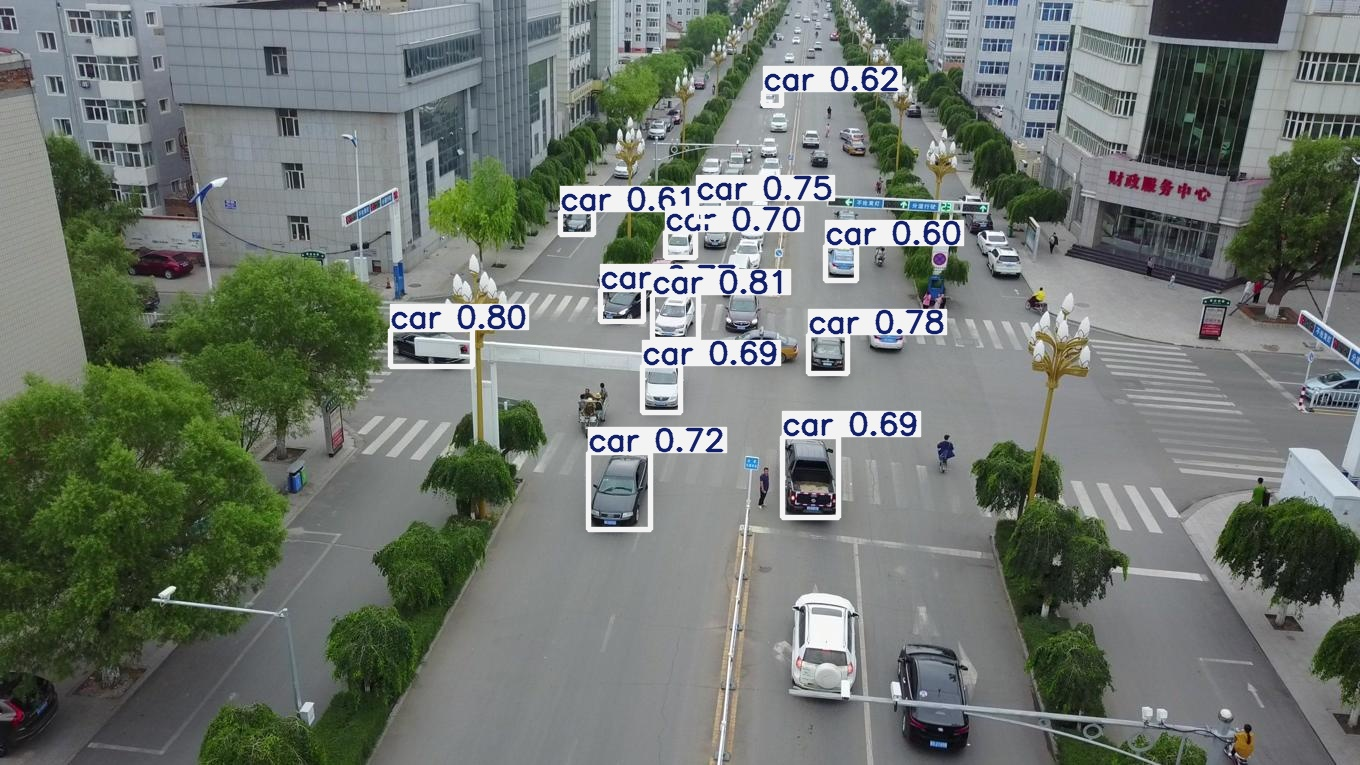
\includegraphics[scale=0.3]{gambar/coco_1.jpg}
    % Keterangan gambar yang diinputkan
    \caption{Proses Deteksi dengan dataset COCO}
    % Label referensi dari gambar yang diinputkan
    \label{fig:deteksi_kendaraan_coco1}
  \end{figure}
  
  Namun, pada implementasinya nanti posisi kamera seharusnya tidak seperti pada gambar \ref{fig:deteksi_kendaraan_coco1}, sehingga dicoba dilakukan deteksi dengan sudut pandang lain yang lebih sesuai. 
  \begin{figure} [H] \centering
      % Nama dari file gambar yang diinputkan
      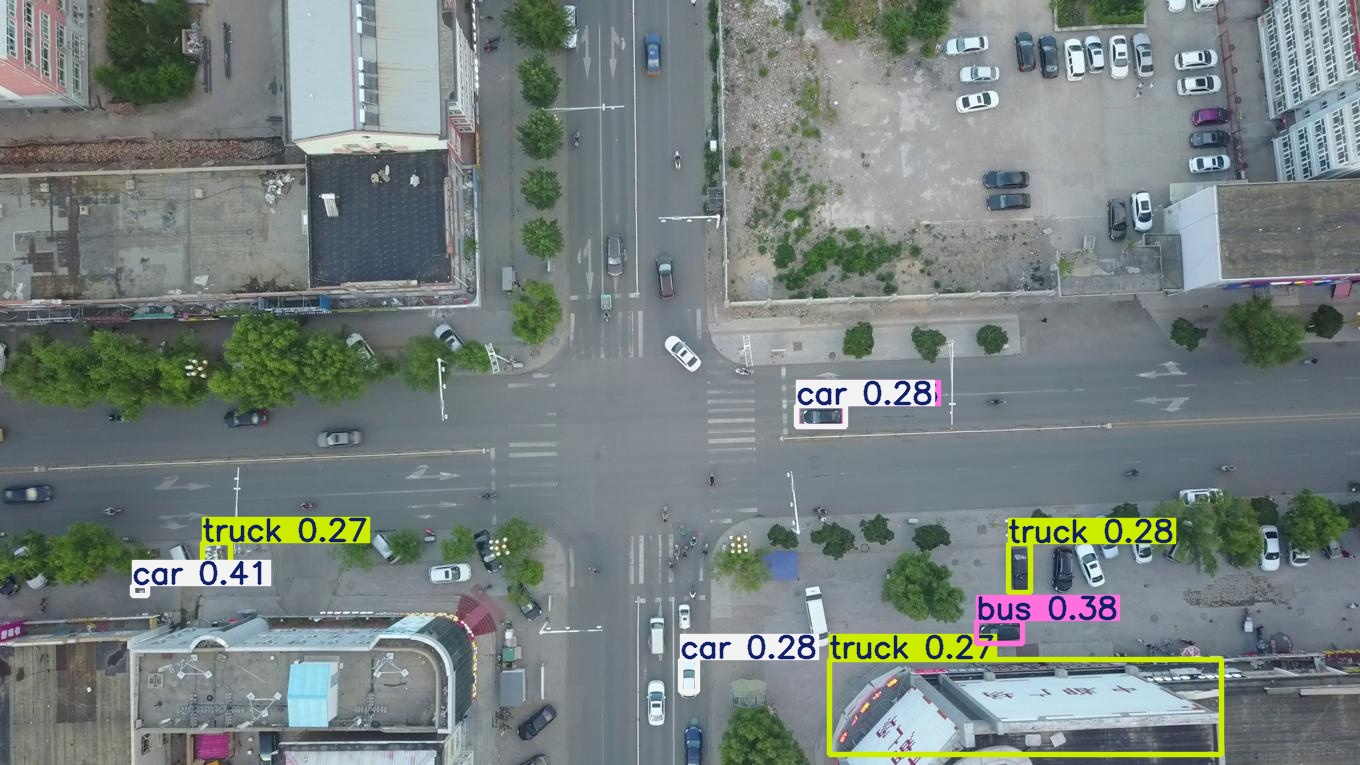
\includegraphics[scale=0.3]{gambar/coco_2.jpg}
      % Keterangan gambar yang diinputkan
      \caption{Proses Deteksi dengan dataset COCO dengan \emph{angle} lebih sesuai}
      % Label referensi dari gambar yang diinputkan
      \label{fig:deteksi_kendaraan_coco2}
    \end{figure}
    
Dikarenakan dataset COCO yang kurang sesuai dengan pengaplikasian yang dimaksudkan pad penelitian ini, penulis mencoba melakukan trainig dengan dataset VisDrone. Penulis melalui proses \emph{labelling}, \emph{pre-processing}, hingga \emph{training} sesuai keterangan di bab 3 Metodologi. Hasil dari model yang di training tersebut seperti berikut.
\begin{figure} [H] \centering
    % Nama dari file gambar yang diinputkan
    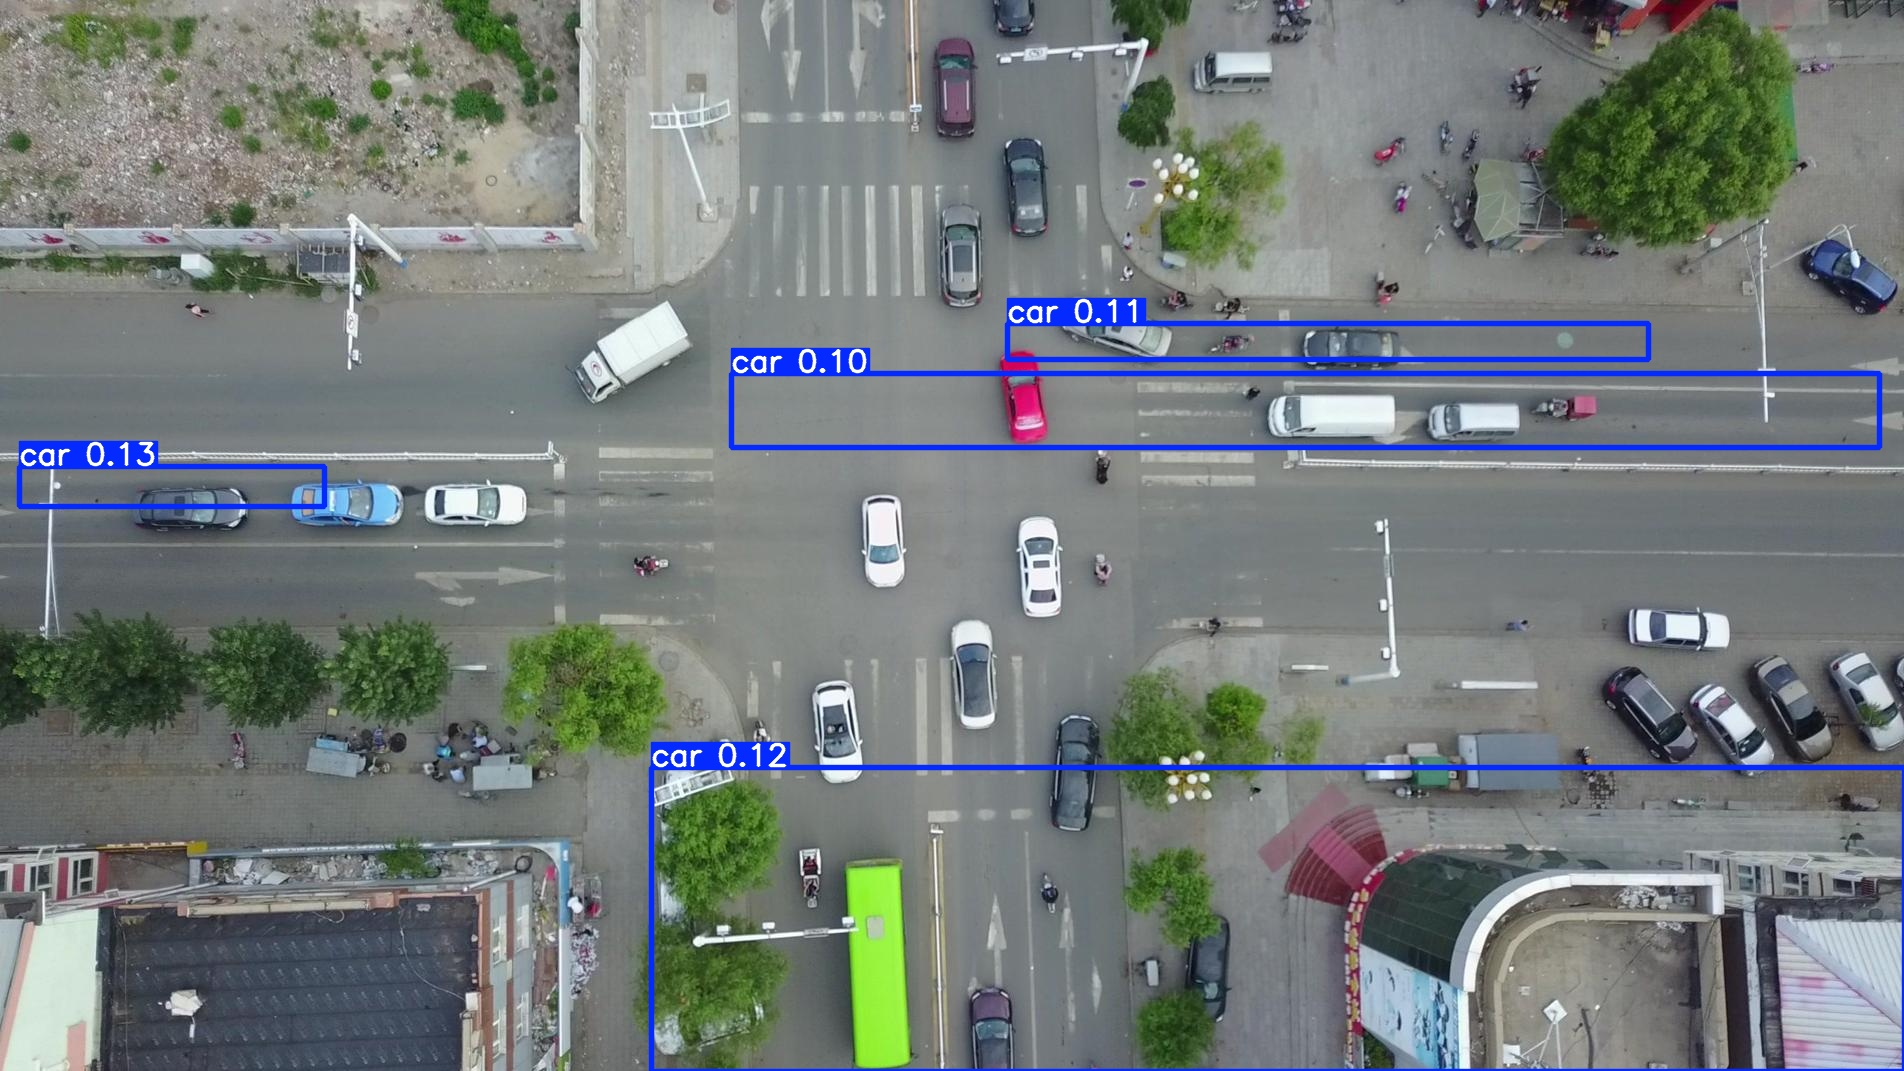
\includegraphics[scale=0.2]{gambar/custom_model.jpg}
    % Keterangan gambar yang diinputkan
    \caption{Proses Deteksi dengan dataset VisDrone}
    % Label referensi dari gambar yang diinputkan
    \label{fig:deteksi_kendaraan_visdrone}
    \end{figure}

Performa yang didapatkan masih belum memenuhi kebutuhan penelitian. Evaluasi dan koreksi harus dilakukan untuk mendapatkan performa model yang diinginkan sesuai dengan kebutuhan penelitian. Meskipun demikian, penulis berkomitmen untuk meneruskan prosedur yang sudah direncanakan agar penelitian ini dapat berjalan sesuai rencana.